\documentclass[10pt,a4paper,twocolumn]{extarticle}

% Submission metadata for the current team entry.
\newcommand{\ReportTitle}{Technical Report}
\newcommand{\ReportTeam}{MLeCDanBGold}
\newcommand{\ReportAuthors}{Khang P. Nguyen, Phuc V. Quang, Huy N. H. Le, Huy N. D. Truong, Phuong D. Nguyen}
\newcommand{\ReportAffiliation}{Ho Chi Minh University of Science - VNUHCM}
\newcommand{\ReportContact}{nguyenphuc.khang110806@gmail.com}
\newcommand{\ReportRevision}{9 September 2026}

% Shared typography and figure vocabulary for the HCMAI technical report.
\usepackage[T1]{fontenc}
\usepackage[utf8]{inputenc}
\usepackage{lmodern}
\usepackage{microtype}
\usepackage[a4paper,top=16mm,bottom=18mm,left=16mm,right=16mm,columnsep=6mm]{geometry}
\usepackage{amsmath,amssymb,bm,mathtools}
\usepackage{booktabs,tabularx,array,multirow,longtable}
\usepackage{enumitem}
\usepackage{graphicx}
\usepackage{float}
\usepackage{caption}
\usepackage{subcaption}
\usepackage{tikz}
\usetikzlibrary{arrows.meta,backgrounds,calc,decorations.pathreplacing,fit,matrix,positioning,shapes.geometric}
\usepackage[numbers,sort&compress]{natbib}
\usepackage{balance}
\usepackage{etoolbox}
\usepackage{titlesec}
\usepackage{fancyhdr}
\usepackage{xcolor}
\usepackage[hidelinks]{hyperref}

% Validated light-mode categorical palette from the report visualization system.
% Every colored object also carries a text label or distinct shape.
\definecolor{ReportBlue}{HTML}{2A78D6}
\definecolor{ReportOrange}{HTML}{EB6834}
\definecolor{ReportAqua}{HTML}{1BAF7A}
\definecolor{ReportInk}{HTML}{0B0B0B}
\definecolor{ReportSecondary}{HTML}{52514E}
\definecolor{ReportMuted}{HTML}{898781}
\definecolor{ReportGrid}{HTML}{E1E0D9}
\definecolor{ReportSurface}{HTML}{FCFCFB}
\definecolor{ReportBlueTint}{HTML}{EAF3FD}
\definecolor{ReportOrangeTint}{HTML}{FDEEE8}
\definecolor{ReportAquaTint}{HTML}{E7F7F1}

\hypersetup{
  colorlinks=true,
  linkcolor=ReportBlue,
  citecolor=ReportBlue,
  urlcolor=ReportBlue,
  pdftitle={HCMAI 2026 Multimodal Video Retrieval Technical Report},
  pdfsubject={System architecture, retrieval, temporal alignment, interface, and deployment}
}

\setlength{\parindent}{0.9em}
\setlength{\parskip}{0pt}
\setlength{\columnsep}{6mm}
\setlength{\abovedisplayskip}{4pt plus 1pt minus 1pt}
\setlength{\belowdisplayskip}{4pt plus 1pt minus 1pt}
\setlength{\abovedisplayshortskip}{2pt plus 1pt}
\setlength{\belowdisplayshortskip}{3pt plus 1pt}
\setlist{nosep,leftmargin=*,topsep=2pt}
\captionsetup{font=small,labelfont=bf,skip=4pt}
\titlespacing*{\section}{0pt}{5.5pt plus 1pt minus 1pt}{2.5pt}
\titlespacing*{\subsection}{0pt}{4pt plus 1pt minus 1pt}{1.5pt}
\titleformat{\section}{\bfseries\normalsize}{\thesection.}{0.45em}{}
\titleformat{\subsection}{\bfseries\small}{\thesubsection}{0.4em}{}

\pagestyle{fancy}
\fancyhf{}
\fancyhead[L]{\footnotesize HCMAI 2026 Technical Report}
\fancyhead[R]{\footnotesize \ReportRevision}
\fancyfoot[C]{\footnotesize \thepage}
\renewcommand{\headrulewidth}{0.3pt}
\setlength{\headheight}{11pt}

\newcommand{\systemname}{\textsc{HCMAI}}
\newcommand{\FrameContext}{\textsc{FrameContext}}
\newcommand{\KIS}{\textsc{KIS}}
\newcommand{\TRAKE}{\textsc{TRAKE}}
\newcommand{\FAISS}{\textsc{Faiss}}
\newcommand{\code}[1]{\texttt{#1}}
\newcommand{\pathcode}[1]{\nolinkurl{#1}}
\newcommand{\vect}[1]{\bm{#1}}
\newcommand{\R}{\mathbb{R}}

% Figure/table guard: the four-page body is intentionally text and equations only.
\newif\ifreportappendix
\reportappendixfalse
\newcommand{\RequireReportAppendix}{%
  \ifreportappendix\else
    \PackageError{hcmai-report}{Figures and tables are restricted to the appendix}%
      {Move this float after \string\appendix.}%
  \fi
}
\AtBeginEnvironment{figure}{\RequireReportAppendix}
\AtBeginEnvironment{figure*}{\RequireReportAppendix}
\AtBeginEnvironment{table}{\RequireReportAppendix}
\AtBeginEnvironment{table*}{\RequireReportAppendix}

% TikZ vocabulary. Color is never the only carrier: every node is labeled and
% each layer uses a distinct shape/border treatment.
\tikzset{
  flowarrow/.style={-{Latex[length=2.1mm,width=1.4mm]},line width=0.75pt,draw=ReportSecondary},
  dataarrow/.style={flowarrow,dashed},
  layer/.style={draw=ReportGrid,rounded corners=2pt,fill=ReportSurface,inner sep=4pt},
  client/.style={draw=ReportBlue,line width=0.9pt,rounded corners=2pt,fill=ReportBlueTint,align=center,minimum height=8mm,font=\small\bfseries},
  service/.style={draw=ReportOrange,line width=0.9pt,rounded corners=2pt,fill=ReportOrangeTint,align=center,minimum height=8mm,font=\small\bfseries},
  artifact/.style={draw=ReportAqua,line width=0.9pt,fill=ReportAquaTint,align=center,minimum height=8mm,font=\small\bfseries},
  process/.style={draw=ReportSecondary,line width=0.75pt,rounded corners=2pt,fill=white,align=center,minimum height=7mm,font=\small},
  note/.style={align=left,font=\footnotesize,text=ReportSecondary},
  callout/.style={circle,fill=ReportBlue,draw=white,line width=0.8pt,text=white,font=\bfseries\scriptsize,minimum size=5.2mm,inner sep=0pt}
}

\newcommand{\screenshotplaceholder}[2]{%
  \IfFileExists{#1}{\includegraphics[width=#2]{#1}}{%
    \fcolorbox{ReportGrid}{ReportSurface}{%
      \parbox[c][0.46\textwidth][c]{#2}{\centering\small\color{ReportMuted}
        Live screenshot pending\\[2pt]\code{#1}}}%
  }%
}

\newcommand{\calloutlabel}[1]{\textbf{[#1]}}


\begin{document}

% The full-width title and abstract count toward the four-page body.
\twocolumn[
  \begin{center}
    {\LARGE\bfseries \ReportTitle\par}
    \vspace{3pt}
    {\normalsize \ReportAuthors\quad---\quad\ReportTeam\par}
    {\small \ReportAffiliation\quad\textbullet\quad\ReportContact\par}
    \vspace{2pt}
    {\footnotesize Ho Chi Minh City AI Challenge 2026 \quad\textbullet\quad \ReportRevision\par}
  \end{center}
  \vspace{2pt}
  \begin{minipage}{0.96\textwidth}
    \small
    \textbf{Abstract---}
    We present an interactive multimodal video-retrieval system for Known Item
    Search (\KIS) and Temporal Retrieval and Alignment of Key Events (\TRAKE).
    A C++/FFmpeg sampler extracts a canonical 1-FPS frame corpus, which specialist
    models enrich with scene context, visible text, objects, speech, and speakers.
    Qwen3-VL, Florence-2, YOLOE, Qwen3-ASR, and pyannote produce this evidence;
    SigLIP2 embeds images and visual-language queries, and BGE-M3 embeds serialized
    \FrameContext{} and speech segments. Exact inner-product \FAISS{} indexes store
    L2-normalized visual, context, and ASR vectors. A fielded BM25 index retains
    literal title, caption, OCR, and ASR matches. Detached frame search combines
    returned lists with weighted reciprocal-rank fusion. \KIS{} and \TRAKE{} instead
    score each event against the full corpus, calibrate and fuse available evidence
    at each frame, then decode strict chronological paths with a linear-time
    monotonic dynamic program. The React client provides search, evidence
    inspection, frame-accurate video navigation, history replay, and a
    revision-aware shared submission workspace. Offline GPU jobs and optional
    inference services run on disposable Thunder Compute instances; canonical
    metadata, indexes, and collaborative state remain local or in S3.
  \end{minipage}
  \vspace{5pt}
]

\label{body:first}
% Main-body claims are grounded in the current implementation and materialized
% manifests. Figures and tables are intentionally deferred to the appendix.

\section{System Overview}

\textbf{MLeCDanBGold} is organized around a canonical frame corpus rather than around its
user interface (Appendix Fig.~\ref{fig:architecture}). Offline preparation imports
or extracts keyframes, enriches them with specialist evidence, constructs dense and
sparse indexes, validates identity/coverage, and publishes immutable bundles. The
online backend opens those artifacts once and composes retrieval, temporal decoding,
canonical materialization, filtering, media resolution, and operator state. The
React application is intentionally a thin inspection and submission client; it does
not own embeddings, corpus identity, ranking, or competition-coordinate conversion.

The design keeps representation, scoring, and task semantics separate. The corpus
layer is authoritative for frames and evidence; modality retrievers own encoders and
index-native search; evidence scorers construct calibrated event--frame matrices;
the temporal package decodes numerical paths; and KIS/TRAKE workflows decide how a
path becomes a response. Consequently a decoder cannot invent a frame, a model
adapter cannot rewrite \code{frame\_idx}, and an unavailable optional modality is
reported as reduced capability rather than replaced by an implicit online rebuild.

The current materialized snapshot is \code{custom-raw1fps-v1}: 873 videos and
470{,}804 canonical frames sampled at one-second targets. It includes 470{,}804
caption, OCR-summary, object-summary, and \FrameContext{} rows; 2{,}689{,}621 OCR
regions; 5{,}654{,}993 object detections; and 40{,}156 speech segments. These are
artifact counts, not retrieval-quality measurements. The same frame contract can
instead ingest organizer-provided keyframes and their authoritative mapping
without re-extraction. In either route, \code{video\_id}, internal
\code{frame\_id}, submission coordinate \code{frame\_idx}, and
\code{timestamp\_ms} remain distinct. No layer derives a competition coordinate
from filename order or a vector-array position.

Appendix Table~\ref{tab:models} lists the model roles. Qwen3-VL-8B produces
captions; Florence-2 reads visible text; YOLOE detects open-vocabulary objects;
Qwen3-ASR-1.7B and pyannote provide timestamped speech and speakers. Retrieval
uses SigLIP2 for images and visual text, and BGE-M3 for context and ASR
text~\cite{qwen3vlcard,florence2,yoloe,qwen3asrcard,pyannote,siglip2,bgem3}.
Qwen3-4B optionally prepares query candidates~\cite{qwen34bcard}; candidate
selection is an explicit client step, not an implicit mutation of a submitted
query. Although the inference package contains an experimental VLM reranker, it
is not wired into the current public \KIS/\TRAKE{} request path and is therefore
not presented as an active stage.

\section{Backend Construction and Execution}

The backend is assembled once from checked configuration and typed artifact
contracts. Startup first opens the canonical \code{frames.parquet} and available
caption, OCR, object, transcript, and media metadata; it then loads the required
visual index and independently attempts the frame-context, ASR-segment, and BM25
bundles. Compatibility checks compare embedding dimensions, canonical mappings,
dataset identities, and model contracts before a source can participate. The
resulting capability map distinguishes frame-native dense evidence, interval-native
speech evidence, and field-native lexical evidence. Large corpus preparation and
index construction never occur in this serving process.

A single \code{SearchService} owns the resulting object graph. Its retrieval service
binds each index to the matching query encoder, projection rule, cache, and fusion
configuration. Its temporal evidence service reuses those bindings to score complete
canonical matrices rather than detached shortlists. Deterministic planners and task
workflows sit above those numerical services, while canonical corpus resolvers and
materializers sit below the response boundary. Filtering is backed by a separate
literal-evidence view, and media/history/submission state cannot alter ranking
artifacts. This composition avoids reopening multi-gigabyte bundles per request and
keeps every transformation testable at a typed boundary.

Execution follows one auditable sequence. Input is validated and converted to one
or more ordered event queries; an explicitly chosen rewrite may change encoder text,
but the original remains available to lexical scoring and explanation. Compatible
queries are batch-encoded, independent components may score concurrently, and all
results retain source identity and coverage. Detached search projects results to
canonical frames before rank fusion. Temporal tasks instead form per-event full-corpus
scores, partition them by video, decode and rank paths, and only then materialize
human-readable evidence and submission coordinates from the FrameStore. Bounded
embedding/thumbnail caches reduce repeated model and image work without caching
mutable response objects or changing deterministic ordering.

\section{Retrieval System}

\subsection{Canonical preparation and FrameContext}

For raw video, the C++/FFmpeg sampler defines target time
$T_k=k\Delta$ with $\Delta=1000\,$ms and $0\leq T_k<D$. When decoding crosses
$T_k$, it emits whichever of the preceding and current decoded timestamps is
closer; a tie selects the preceding frame. Thus a video of duration $D$ yields
$\lceil D/\Delta\rceil$ samples without assuming constant decode cadence. The
custom submission coordinate is
\begin{equation}
 f_k=\left\lfloor \left\lceil\overline{r}\right\rceil
                 \frac{T_k}{1000}\right\rfloor ,
 \label{eq:frame-coordinate}
\end{equation}
where $\overline{r}$ is average FPS. Extraction validates counts and identity,
then atomically publishes durable 1024-pixel JPEGs and higher-quality enrichment
images. Organizer data follows a separate lossless route: supplied keyframes are
sorted by mapping order and
$\texttt{timestamp\_ms}=\operatorname{round}(1000\,\texttt{pts\_time})$;
supplied \code{frame\_idx} remains authoritative. Both routes
converge on the same canonical schema (Appendix Fig.~\ref{fig:preparation}).

Custom preparation is resumable and batch-bounded. A sorted source manifest and
extraction configuration receive a SHA-256 identity before work starts. Each
batch stages source/archive data, extracts frames, runs caption/OCR/object
specialists, builds \FrameContext, encodes visual/context vectors, validates or
reuses timestamped ASR, projects per-video artifacts, and atomically commits a
three-index handoff before scratch cleanup. Durable images feed captioning,
objects, and visual embeddings; the higher-quality enrichment variant feeds OCR.
A batch is not marked enriched merely because files exist: specialist tables must
cover the expected canonical frames and pass identity checks. This order avoids
publishing embeddings whose text or image lineage cannot be reconstructed.

Caption, OCR, and object stages retain their specialist artifacts. A deterministic
\FrameContext{} view serializes only valid evidence in the order
\code{[CAPTION]}, \code{[VISIBLE\_TEXT]}, \code{[OBJECTS]}, separated by blank
lines. Budgets are 80, 80, and 40 whitespace tokens, respectively; OCR text is
included only when quality is at least 0.5. Captions must be complete and
error-free, OCR must additionally be non-empty and pass that quality gate, and
objects require a completed non-empty summary. Raw OCR quality and object count
remain recorded even when their text is excluded. Availability, OCR quality, object
count, source versions, and frame-store lineage remain typed fields even when a
text section is omitted. The builder performs a bounded SQLite join, checks
source manifests and canonical identities, and atomically publishes Parquet plus
manifest output. Consequently the combined text can be rebuilt without
sacrificing source-level inspection.

\subsection{Indexes and two fusion regimes}

SigLIP2 encodes every durable image into a 768-dimensional vector and BGE-M3
encodes \FrameContext{} and non-empty ASR segments into 1024 dimensions. All
vectors are float32 and L2-normalized, so exact inner product equals cosine
similarity. The frame-native bundles use \FAISS{} \code{IndexFlatIP}; each also
stores its vector matrix, canonical mapping, timestamps, and per-video posting
arrays~\cite{faiss}. For a batch of event queries $Q$ and corpus vectors $V$,
full temporal scoring is the chunked matrix product
\begin{equation}
 S^{(m)}=Q^{(m)}{V^{(m)}}^{\!\top}.
 \label{eq:dense-score}
\end{equation}
The ASR index is segment-native: a half-open interval $[a,b)$ contributes its
maximum score to covered canonical frames, with a bounded nearest-midpoint
fallback only in detached top-$K$ projection.

A dense bundle is self-describing: \code{dense.index} is accompanied by
\code{vectors.npy}, canonical frame or segment mapping, metadata, timestamps, and
compact per-video posting offsets/positions. Build preflight checks frame-store
authority, expected coverage, model/index contracts, and source lineage before
encoding. Online top-$K$ search delegates to \FAISS; full-corpus or video-subset
temporal scoring deliberately reads the normalized vector matrix and computes
Eq.~\ref{eq:dense-score} in bounded chunks. This avoids approximating event
alignment from a shortlist and lets the same canonical ordering split scores by
video without a second identity join. Queries sharing an encoder family are
batch-encoded, while independent modality searches can run concurrently.

For segment search, results first retain the strongest segment contribution per
frame. Canonical frames inside $[a,b)$ are preferred; only an empty interval uses
the nearest segment midpoint, and then only within the configured 5000-ms bound.
Ties resolve by distance, timestamp, frame index, and frame ID. Temporal
full-corpus projection is stricter: covered frames receive the maximum of all
overlapping interval scores and uncovered positions carry both score zero and a
false coverage mask, later consumed by Eq.~\ref{eq:adaptive-fusion}.

A sparse index independently stores BM25 matrices for title, caption, OCR, and
ASR after Unicode NFKC normalization, lowercasing, and alphanumeric tokenization.
With $k_1=1.5$ and $b=0.75$, a query-term contribution is
\begin{equation}
 \begin{aligned}
  K_d&=k_1\!\left(1-b+b|d|/\overline{|d|}\right),\\
  s_q(d)&=\operatorname{idf}(q)\,
    \frac{tf(q,d)(k_1+1)}{tf(q,d)+K_d},\\
  \operatorname{idf}(q)&=\log\!\left(1+
    \frac{N-df(q)+0.5}{df(q)+0.5}\right).
 \end{aligned}
 \label{eq:bm25}
\end{equation}
following the probabilistic relevance framework~\cite{bm25}. The current snapshot
has populated title, OCR, and ASR vocabularies; its serialized BM25 caption field
is empty, while semantic caption evidence remains present through
\FrameContext{}. Appendix Table~\ref{tab:artifacts} records this manifest state.
Sparse scoring sums the selected query-token columns rather than densifying the
entire vocabulary. Original event text queries title, OCR, and ASR fields;
caption-oriented retrieval text may address the caption field. This separation
retains literal names, signs, and spoken phrases that a dense embedding can
smooth over, while preventing a synthetic combined context string from being
misreported as a source caption.

The implementation deliberately has two non-interchangeable fusion regimes.
For detached nearest-neighbor frame search, modality lists are combined by
weighted reciprocal-rank fusion~\cite{rrf}:
\begin{equation}
 R(i)=\sum_{m\in\mathcal{M}_i}\frac{w_m}{60+\operatorname{rank}_m(i)}.
 \label{eq:rrf}
\end{equation}
This is rank-only, works on the union of returned frame IDs, and preserves source
provenance. One-based ranks, active-weight normalization, a required visual
source, and deterministic tie-breaking (fused score, best source rank, then frame
ID) make repeated queries stable. ASR segments are projected before fusion, so
all list members already carry canonical frame identity. RRF should not be
described as the temporal \KIS/\TRAKE{} scorer.

Temporal search instead scores every event against every canonical frame. For
component $m$ and event $e$, supported values are quantile-clipped and min--max
mapped to $\widehat{S}_{met}\in[0,1]$. Dense reliability measures upper-tail
contrast,
\begin{equation}
 z_{me}=\frac{\max(\mu^{\mathrm{top}}_{me}-\operatorname{med}_{me},0)}
 {\operatorname{IQR}_{me}+\varepsilon},\qquad
 \rho_{me}=\frac{z_{me}}{1+z_{me}},
 \label{eq:reliability}
\end{equation}
whereas a lexical row has binary reliability when any exact match exists. A
deterministic cue router adjusts base weights for speech, visible-text, or visual
language. Coverage $c_{met}\in\{0,1\}$ then prevents absent segment/evidence data
from diluting a score:
\begin{equation}
 F_{et}=\frac{\sum_m w_{me}\rho_{me}c_{met}\widehat{S}_{met}}
                   {\sum_m w_{me}\rho_{me}c_{met}},
 \quad w_{me}=w_m^{0}\,g_m(q_e).
 \label{eq:adaptive-fusion}
\end{equation}
If no nonvisual component covers a frame, calibrated visual evidence supplies the
fallback. The robust defaults use the 5th percentile and maximum as calibration
bounds, the strongest one percent capped at 128 frames for $\mu^{\mathrm{top}}$,
and $\varepsilon=10^{-6}$. Base masses are 0.35 visual, 0.35 context, 0.08 dense
ASR, and 0.02/0.10/0.04/0.06 for title/caption/OCR/ASR BM25. Cue multipliers are
1.4 for visual language, 5.0 for speech, and 3.0 for visible text; Eq.~\ref{eq:adaptive-fusion}
renormalizes the resulting positive mass at every frame. These are deterministic
policies, not learned weights.

This local renormalization makes missing evidence distinct from weak
evidence and produces one fused event--frame matrix per video.

\subsection{KIS/TRAKE temporal orchestration}

\KIS{} first converts a natural-language description into ordered moments using
a deterministic Vietnamese-aware planner; explicitly selected query-preparation
candidates may replace only retrieval text, while original text remains available
to BM25. \TRAKE{} accepts the ordered events directly. Both call the same temporal
service: build component matrices, calibrate and fuse them, split the canonical
matrix by video, decode paths, and revalidate every identity before response
materialization (Appendix Fig.~\ref{fig:temporal}).

The planner prefers non-empty lines, then sentence boundaries; removes a trailing
question; folds attribute/enumeration sentences into the preceding moment; and
recognizes Vietnamese/English transition cues. A ``before that'' moment is moved
before the event it references, whereas later cues preserve forward order. The
planner is intentionally deterministic so UI replay and lexical evidence can show
exactly what was aligned. Request validation bounds the event count at 32 and
rejects an empty sequence before allocating a full-corpus matrix.

For one video, let $F_{et}$ be the fused score for event $e$ at frame $t$ and
$\tau_t$ its timestamp. Strict chronological alignment uses
\begin{align}
 D_{0t}&=F_{0t},\nonumber\\
 D_{et}&=F_{et}+\max_{u<t}\left[D_{e-1,u}
              -\lambda(\tau_t-\tau_u)\right].
 \label{eq:dp}
\end{align}
The gap penalty ($\lambda=10^{-5}$ by default) discourages unnecessarily distant
events without imposing a fixed window. Rewriting the predecessor term as
\begin{equation}
 D_{et}=F_{et}-\lambda\tau_t+
 \max_{u<t}\left(D_{e-1,u}+\lambda\tau_u\right)
 \label{eq:prefix-dp}
\end{equation}
permits a prefix maximum and backpointer scan in $O(ET)$ time and $O(ET)$
backpointer space, rather than $O(ET^2)$. At each position, cumulative maxima
store both the best shifted predecessor value and its canonical position; equal
values deliberately keep the latest position. Endpoints with non-finite state are
unreachable, and a video with fewer admissible frames/score clusters than events
returns no path. If configured, non-negative event scores are exponentiated by an
\code{event\_power} before decoding; the active value 1.0 leaves them unchanged.
Ties choose the latest valid
predecessor. Optional score-profile clusters prevent multiple events from using a
near-identical region. The runtime retains up to five alternatives per video and
suppresses final-event alternatives within 30 seconds before global ranking.

\KIS{} materializes the upper-middle aligned event,
$\lfloor |P|/2\rfloor$, as the representative result while retaining the complete
path for explanation and navigation. \TRAKE{} returns every ordered canonical
frame/timestamp sequence and submits the entire path as one row. This shared
optimizer guarantees consistent temporal semantics between tasks while their
output contracts remain different. Before returning either response, the temporal
service resolves every DP position through the canonical FrameStore and verifies
video ID, frame ID, frame index, and timestamp arrays. \KIS{} then attaches the
representative frame's inspectable metadata plus the full event/frame/timestamp
alignment. \TRAKE{} preserves arrays for every path unchanged. The API therefore
returns competition-facing coordinates and human-readable evidence without
allowing the optimizer's array offsets to escape as identities.

\section{Operator Interface (Brief)}

The interface exposes the backend's task semantics without duplicating them.
Plain text starts \KIS; explicit \code{E1:}, \code{E2:}, \ldots lines start
\TRAKE. Operators select Top-$K$ and dense/lexical families, inspect result cards
and complete alignments, then open a video at the retrieved timestamp with caption,
OCR, object, ASR, and canonical-coordinate evidence beside it. Appendix
Figs.~\ref{fig:ui-kis}--\ref{fig:ui-player} show these interactions directly.

A compact collaborative workspace provides user-scoped query replay, manual
video/timestamp opening, and shared CSV answer files (Fig.~\ref{fig:ui-workspace}).
SQLite stores revisions and committed rows; synchronization distributes only
revision-aware file commands. \KIS{} appends one video/frame pair, whereas
\TRAKE{} appends the complete ordered path as one row. The UI supports editing,
validation, and ZIP export, but does not claim chat, shared cursors, or presence.

\section{Thunder Compute Execution Boundary}

The maintained index-build runbook uses one RTX A6000 as an ephemeral worker.
It inventories or downloads only canonical frames, keyframes, \FrameContext{},
and transcripts from S3; produces visual, context, and ASR-segment bundles; runs
coverage/identity validation; and publishes a checksummed version only when its
build report passes. Separately, an operator may create a disposable GPU VM,
copy the selected inference package, run one Uvicorn worker on private port 8100,
and expose it through a protected Cloudflare endpoint. GPU SKU is an operational
choice (the checked-in example uses an L40), not a retrieval invariant. No
tracked launcher claims automatic lifecycle management: instance creation,
upload, health checking, and deletion remain explicit operator steps. The local
FastAPI service and S3 artifacts therefore survive VM teardown~\cite{thunder}.

\section{Scope and Reproducibility}

This report describes the current implementation and materialized custom-corpus
snapshot, not the proposed VLM-reranking design or a quantitative benchmark.
Configuration pins model revisions, but the checked-out visual/context index
metadata omit some revision or source/config fingerprints, and no promoted
\code{build\_report.json} accompanies this local bundle. Those omissions do not
change the algorithms above; they do mean an official release should regenerate
or reconcile manifests before claiming immutable end-to-end provenance. The
appendix records the exact observed state and maps each presented subsystem to a
diagram, table, or live UI capture.

\vspace{-4pt}
\balance
\label{body:last}

% Enforce the four-page title-through-body limit before references and the
% appendix begin on a new page.
\ifnum\value{page}>4
  \PackageError{hcmai-report}{Main body exceeds the four-page limit}%
    {Shorten sections/main-body.tex; references and appendices are excluded.}%
\fi

\clearpage
\addcontentsline{toc}{section}{References}
\bibliographystyle{unsrtnat}
\bibliography{references}

\clearpage
\onecolumn
\appendix
\reportappendixtrue
\section{Architecture and Component Map}

\begin{figure}[htbp]
\centering
\resizebox{0.98\textwidth}{!}{%
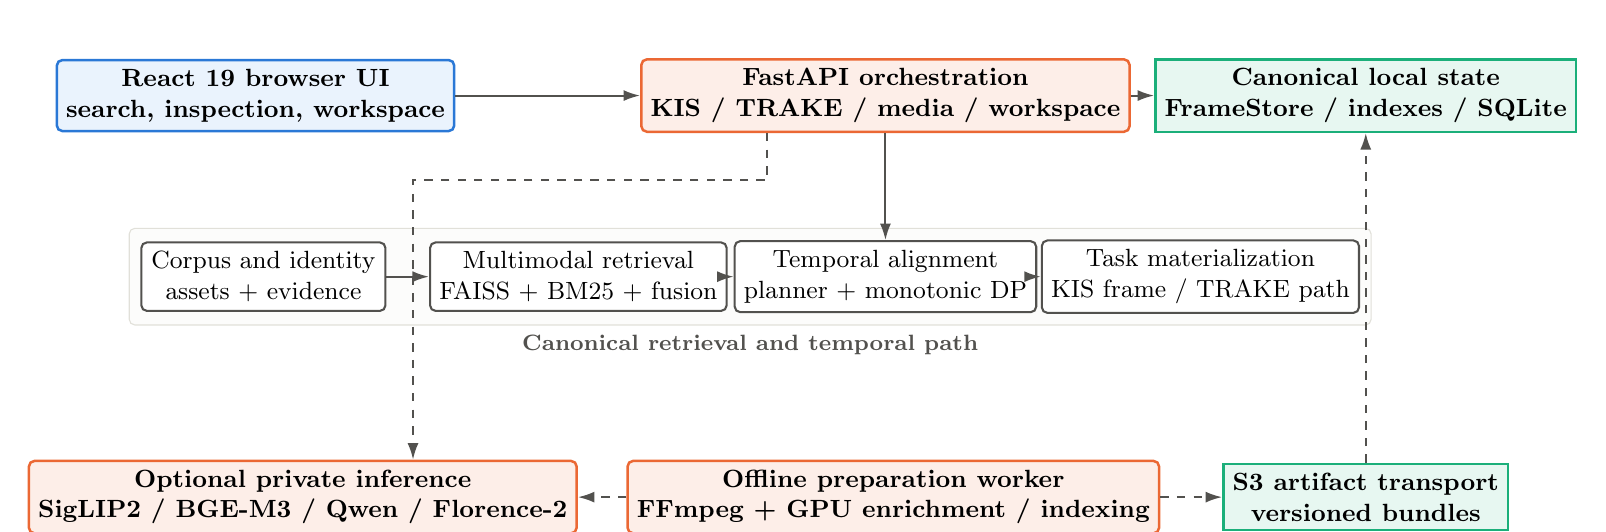
\begin{tikzpicture}[x=1mm,y=1mm]
  % Operator and serving boundary.
  \node[client,minimum width=40mm] (browser) at (24,58)
    {React 19 browser UI\\search, inspection, workspace};
  \node[service,minimum width=50mm] (api) at (104,58)
    {FastAPI orchestration\\KIS / TRAKE / media / workspace};
  \node[artifact,minimum width=39mm] (state) at (165,58)
    {Canonical local state\\FrameStore / indexes / SQLite};

  % Canonical online execution path.
  \node[process,minimum width=31mm] (corpus) at (25,35)
    {Corpus and identity\\assets + evidence};
  \node[process,minimum width=33mm] (retrieval) at (65,35)
    {Multimodal retrieval\\FAISS + BM25 + fusion};
  \node[process,minimum width=35mm] (temporal) at (104,35)
    {Temporal alignment\\planner + monotonic DP};
  \node[process,minimum width=34mm] (materialize) at (144,35)
    {Task materialization\\KIS frame / TRAKE path};

  % Replaceable compute and artifact-publication boundary.
  \node[service,minimum width=48mm] (gpu) at (30,7)
    {Optional private inference\\SigLIP2 / BGE-M3 / Qwen / Florence-2};
  \node[service,minimum width=50mm] (offline) at (105,7)
    {Offline preparation worker\\FFmpeg + GPU enrichment / indexing};
  \node[artifact,minimum width=34mm] (s3) at (165,7)
    {S3 artifact transport\\versioned bundles};

  \draw[flowarrow] (browser) -- (api);
  \draw[flowarrow] (api) -- (state);
  \draw[flowarrow] (api.south) -- (temporal.north);
  \draw[flowarrow] (corpus) -- (retrieval);
  \draw[flowarrow] (retrieval) -- (temporal);
  \draw[flowarrow] (temporal) -- (materialize);

  \draw[dataarrow] ([xshift=-15mm]api.south) -- ++(0,-6mm)
    -| ([xshift=14mm]gpu.north);
  \draw[dataarrow] (offline) -- (gpu);
  \draw[dataarrow] (offline) -- (s3);
  \draw[dataarrow] (s3.north) -- (state.south);

  \begin{scope}[on background layer]
    \node[layer,fit=(corpus)(retrieval)(temporal)(materialize),
      label={[font=\footnotesize\bfseries,text=ReportSecondary]
      below:Canonical retrieval and temporal path}] {};
  \end{scope}
\end{tikzpicture}%
}
\caption{System architecture and trust boundary. Solid arrows are online control/data flow; dashed arrows are optional inference or artifact transport. Retrieval state is local and canonical; the GPU service is replaceable. Every box has a distinct label and border in addition to color.}
\label{fig:architecture}
\end{figure}

\begin{table}[htbp]
\centering
\caption{Implemented model and algorithm inventory. ``Active'' means present in the documented preparation or online path; optional services are never implied to be mandatory at serving time.}
\label{tab:models}
\small
\begin{tabularx}{\textwidth}{@{}>{\bfseries}p{0.15\textwidth}p{0.26\textwidth}Xp{0.12\textwidth}@{}}
\toprule
Capability & Model / algorithm & Produced evidence and downstream use & Status \\
\midrule
Caption & Qwen/Qwen3-VL-8B-Instruct & Frame caption; first \FrameContext{} section and inspectable specialist artifact & Offline active \\
Visible text & Florence-2-base-ft & OCR regions, frame summary, quality; gated \FrameContext{} section and BM25 OCR field & Offline active \\
Objects & YOLOE-26l-seg & Detections and normalized object summary; \FrameContext{} section and literal filter & Offline active \\
Speech & Qwen3-ASR-1.7B-hf & Timestamped transcript segments; BGE-M3 segment index and BM25 ASR field & Offline active \\
Speakers & pyannote community-1 & Diarization attached to transcript segments & Configurable \\
Visual encoder & SigLIP2 base patch16-224 & 768-D image vectors and visual-language query vectors & Active \\
Text encoder & BAAI/bge-m3 & 1024-D \FrameContext{} and ASR-segment vectors & Active \\
Dense search & FAISS \code{IndexFlatIP} & Exact inner product over L2-normalized vectors; cosine-equivalent ranking & Active \\
Lexical search & Fielded BM25 & Title/caption/OCR/ASR literal evidence & Active \\
Query preparation & Qwen/Qwen3-4B & Five optional candidate rewrites selected explicitly by the client & Optional \\
Temporal decoding & Prefix-max monotonic DP & Strict same-video event paths, alternatives, and canonical backpointers & KIS/TRAKE active \\
VLM reranking & Qwen3-VL reranker adapter & Experimental package capability; absent from public request contract and UI & Not wired \\
\bottomrule
\end{tabularx}
\end{table}

\clearpage
\section{Offline Preparation and Index Construction}

\begin{figure}[htbp]
\centering
\resizebox{0.98\textwidth}{!}{%
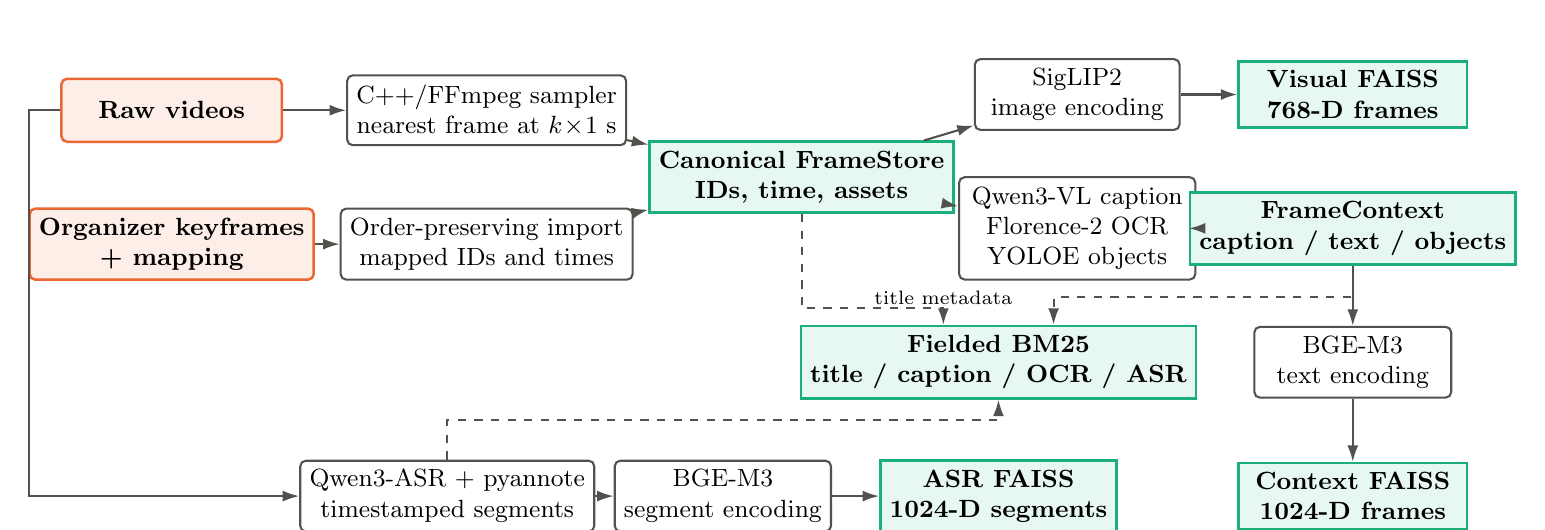
\begin{tikzpicture}[x=1mm,y=1mm]
  % A compact tree uses vertical space so every stage remains readable and
  % connectors never pass through another node.
  \node[service,minimum width=28mm] (raw) at (15,55) {Raw videos};
  \node[service,minimum width=28mm] (provided) at (15,38) {Organizer keyframes\\+ mapping};
  \node[process,minimum width=30mm] (extract) at (55,55)
    {C++/FFmpeg sampler\\nearest frame at $k\!\times\!1$ s};
  \node[process,minimum width=30mm] (import) at (55,38)
    {Order-preserving import\\mapped IDs and times};
  \node[artifact,minimum width=30mm] (frame) at (95,46.5)
    {Canonical FrameStore\\IDs, time, assets};

  \node[process,minimum width=26mm] (siglip) at (130,57) {SigLIP2\\image encoding};
  \node[artifact,minimum width=29mm] (vindex) at (165,57) {Visual FAISS\\768-D frames};
  \node[process,minimum width=30mm,minimum height=13mm] (specialists) at (130,40)
    {Qwen3-VL caption\\Florence-2 OCR\\YOLOE objects};
  \node[artifact,minimum width=28mm] (context) at (165,40)
    {FrameContext\\caption / text / objects};

  \node[artifact,minimum width=32mm] (bm25) at (120,23)
    {Fielded BM25\\title / caption / OCR / ASR};
  \node[process,minimum width=25mm] (contextbge) at (165,23)
    {BGE-M3\\text encoding};
  \node[artifact,minimum width=29mm] (cindex) at (165,6)
    {Context FAISS\\1024-D frames};

  \node[process,minimum width=30mm] (asr) at (50,6)
    {Qwen3-ASR + pyannote\\timestamped segments};
  \node[process,minimum width=25mm] (asrbge) at (85,6)
    {BGE-M3\\segment encoding};
  \node[artifact,minimum width=29mm] (aindex) at (120,6)
    {ASR FAISS\\1024-D segments};

  \draw[flowarrow] (raw) -- (extract);
  \draw[flowarrow] (extract) -- (frame);
  \draw[flowarrow] (provided) -- (import);
  \draw[flowarrow] (import) -- (frame);

  \draw[flowarrow] (frame) -- (siglip);
  \draw[flowarrow] (siglip) -- (vindex);
  \draw[flowarrow] (frame) -- (specialists);
  \draw[flowarrow] (specialists) -- (context);
  \draw[flowarrow] (context) -- (contextbge);
  \draw[flowarrow] (contextbge) -- (cindex);

  \draw[flowarrow] (raw.west) -- ++(-4mm,0) |- (asr.west);
  \draw[flowarrow] (asr) -- (asrbge);
  \draw[flowarrow] (asrbge) -- (aindex);

  \draw[dataarrow] (frame.south) -- ++(0,-12mm)
    -| node[pos=0.70,above,font=\scriptsize]{title metadata}
    ([xshift=-7mm]bm25.north);
  \draw[dataarrow] (context.south) -- ++(0,-4mm)
    -| ([xshift=7mm]bm25.north);
  \draw[dataarrow] (asr.north) -- ++(0,5mm) -| (bm25.south);
\end{tikzpicture}%
}
\caption{Two ingestion routes converge on one canonical frame identity. Solid arrows show model or encoding stages; dashed arrows feed the fielded lexical index. The frame-native visual/context indexes and segment-native ASR index preserve their native evidence geometry rather than forcing all sources into one lossy representation.}
\label{fig:preparation}
\end{figure}

\begin{table}[htbp]
\centering
\caption{Observed materialized artifact snapshot. Counts document system scale, not retrieval effectiveness. Missing provenance fields are reported rather than inferred.}
\label{tab:artifacts}
\small
\begin{tabularx}{\textwidth}{@{}>{\bfseries}p{0.20\textwidth}p{0.15\textwidth}p{0.20\textwidth}X@{}}
\toprule
Artifact & Entities & Representation & Observed contract / caveat \\
\midrule
Canonical FrameStore & 873 videos; 470{,}804 frames & Parquet + manifest; 1-s targets & \code{custom-raw1fps-v1}; no duplicate submission-coordinate groups \\
Caption / OCR / objects / context & 470{,}804 rows each & Specialist Parquet + deterministic \FrameContext{} & 2{,}689{,}621 OCR regions and 5{,}654{,}993 object detections \\
Visual index & 470{,}804 frames & 768-D float32, L2, flat IP & Model name recorded; serialized model revision/source/config fingerprints absent \\
Vietnamese context index & 470{,}804 frames & 1024-D float32, L2, flat IP & Dataset label differs from FrameStore; revision/retrieval-source/fingerprints absent \\
ASR segment index & 40{,}156 intervals & 1024-D float32, L2, flat IP & BGE-M3 revision recorded; half-open temporal geometry retained \\
BM25 index & 470{,}804 documents & Four sparse field matrices & $k_1=1.5$, $b=0.75$; current caption vocabulary size is zero \\
\bottomrule
\end{tabularx}
\end{table}

\begin{table}[H]
\centering
\caption{Key deterministic policies and defaults used in this report.}
\label{tab:parameters}
\small
\begin{tabularx}{\textwidth}{@{}>{\bfseries}p{0.18\textwidth}p{0.26\textwidth}X@{}}
\toprule
Stage & Parameter & Policy \\
\midrule
Sampling & $\Delta=1000$ ms & Select nearest decoded timestamp; ties choose preceding frame; targets lie in $[0,D)$ \\
FrameContext & budgets $80/80/40$; OCR $\geq0.5$ & Ordered caption, visible-text, object sections; preserve lineage and availability \\
Dense bundles & float32, L2, flat IP & Exact cosine-equivalent search; vectors, mappings, postings, and timestamps stored together \\
ASR projection & maximum gap 5000 ms & Prefer frames inside $[a,b)$; otherwise nearest midpoint within bound for detached search \\
Detached fusion & RRF constant 60 & Weighted union of modality top-$K$ lists; visual source required \\
Temporal fusion & adaptive, coverage-aware & Quantile calibration, reliability gating, cue routing, per-frame renormalization \\
Alignment & $\lambda=10^{-5}$; power 1 & Strict monotonic path; prefix-max recurrence; latest predecessor on ties \\
Alternatives & 5 paths/video; 30 s separation & Suppress near-duplicate final-event moments before global ranking \\
\bottomrule
\end{tabularx}
\end{table}

\clearpage
\section{Online Fusion and Temporal Task Orchestration}

\begin{figure}[htbp]
\centering
\resizebox{0.98\textwidth}{!}{%
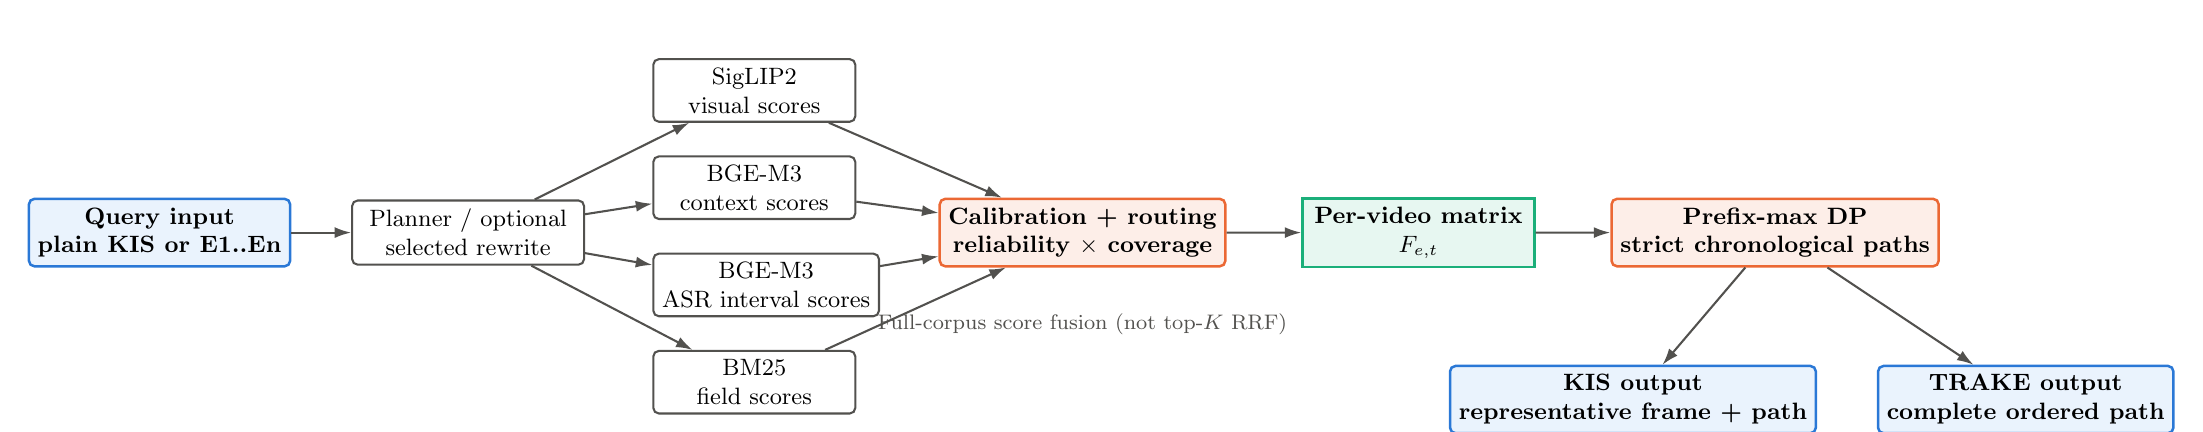
\begin{tikzpicture}[node distance=6mm and 7mm,scale=0.95,transform shape]
  \node[client,minimum width=29mm] (query) {Query input\\plain KIS or E1..En};
  \node[process,minimum width=31mm,right=8mm of query] (plan) {Planner / optional\\selected rewrite};

  \node[process,minimum width=27mm,right=9mm of plan,yshift=19mm] (visual) {SigLIP2\\visual scores};
  \node[process,minimum width=27mm,right=9mm of plan,yshift=6mm] (context) {BGE-M3\\context scores};
  \node[process,minimum width=27mm,right=9mm of plan,yshift=-7mm] (asr) {BGE-M3\\ASR interval scores};
  \node[process,minimum width=27mm,right=9mm of plan,yshift=-20mm] (lexical) {BM25\\field scores};

  \node[service,minimum width=36mm,right=11mm of context,yshift=-6mm] (fusion) {Calibration + routing\\reliability $\times$ coverage};
  \node[artifact,minimum width=31mm,right=10mm of fusion] (matrix) {Per-video matrix\\$F_{e,t}$};
  \node[service,minimum width=35mm,right=10mm of matrix] (dp) {Prefix-max DP\\strict chronological paths};

  \node[client,minimum width=30mm,below=13mm of dp,xshift=-19mm] (kis) {KIS output\\representative frame + path};
  \node[client,minimum width=30mm,right=8mm of kis] (trake) {TRAKE output\\complete ordered path};

  \draw[flowarrow] (query) -- (plan);
  \draw[flowarrow] (plan) -- (visual);
  \draw[flowarrow] (plan) -- (context);
  \draw[flowarrow] (plan) -- (asr);
  \draw[flowarrow] (plan) -- (lexical);
  \draw[flowarrow] (visual) -- (fusion);
  \draw[flowarrow] (context) -- (fusion);
  \draw[flowarrow] (asr) -- (fusion);
  \draw[flowarrow] (lexical) -- (fusion);
  \draw[flowarrow] (fusion) -- (matrix);
  \draw[flowarrow] (matrix) -- (dp);
  \draw[flowarrow] (dp) -- (kis);
  \draw[flowarrow] (dp) -- (trake);

  \node[note,below=5mm of fusion,align=center] {Full-corpus score fusion (not top-$K$ RRF)};
\end{tikzpicture}%
}
\caption{Shared KIS/TRAKE online path. Original event text remains available to lexical scoring; any rewrite is explicit. Component support and confidence are applied before the same monotonic decoder produces task-specific materializations.}
\label{fig:temporal}
\end{figure}

\begin{figure}[htbp]
\centering
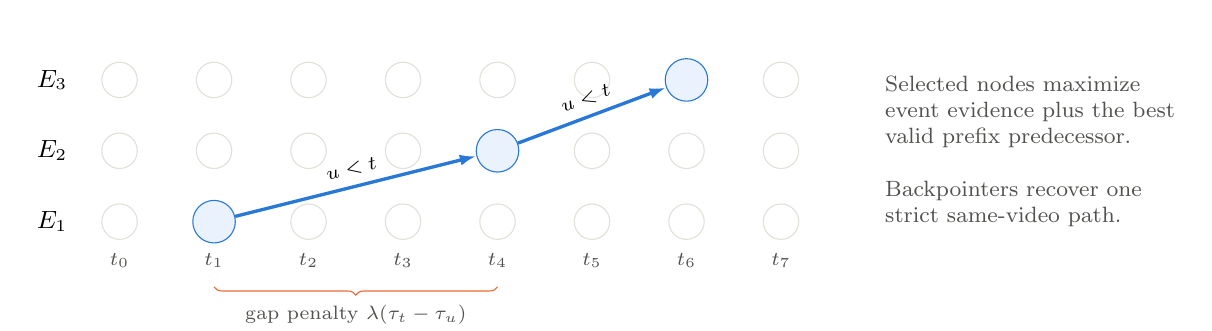
\begin{tikzpicture}[x=12mm,y=9mm]
  \foreach \x/\lab in {0/$t_0$,1/$t_1$,2/$t_2$,3/$t_3$,4/$t_4$,5/$t_5$,6/$t_6$,7/$t_7$}
    \node[font=\scriptsize,text=ReportSecondary] at (\x,-0.55) {\lab};
  \foreach \y/\event in {0/$E_1$,1/$E_2$,2/$E_3$}
    \node[font=\small\bfseries,anchor=east] at (-0.45,\y) {\event};
  \foreach \x in {0,...,7}
    \foreach \y in {0,...,2}
      \node[draw=ReportGrid,circle,minimum size=4.5mm,inner sep=0pt,fill=white] (n\y\x) at (\x,\y) {};
  \node[draw=ReportBlue,fill=ReportBlueTint,circle,minimum size=5.4mm,inner sep=0pt] (p00) at (1,0) {};
  \node[draw=ReportBlue,fill=ReportBlueTint,circle,minimum size=5.4mm,inner sep=0pt] (p11) at (4,1) {};
  \node[draw=ReportBlue,fill=ReportBlueTint,circle,minimum size=5.4mm,inner sep=0pt] (p22) at (6,2) {};
  \draw[flowarrow,draw=ReportBlue,line width=1.2pt] (p00) -- node[above,sloped,font=\scriptsize]{$u<t$} (p11);
  \draw[flowarrow,draw=ReportBlue,line width=1.2pt] (p11) -- node[above,sloped,font=\scriptsize]{$u<t$} (p22);
  \draw[decorate,decoration={brace,amplitude=3pt,mirror},draw=ReportOrange]
    (1,-0.92) -- node[below=3pt,font=\scriptsize,text=ReportSecondary]{gap penalty $\lambda(\tau_t-\tau_u)$} (4,-0.92);
  \node[note,anchor=west] at (8.0,1.55) {Selected nodes maximize\\event evidence plus the best\\valid prefix predecessor.};
  \node[note,anchor=west] at (8.0,0.25) {Backpointers recover one\\strict same-video path.};
\end{tikzpicture}
\caption{Dynamic-programming interpretation. Each event selects a strictly later canonical frame. Prefix maxima replace an all-pairs predecessor search, while backpointers preserve exact frame identity.}
\label{fig:dp-explainer}
\end{figure}

\clearpage
\section{Live Operator Interface}

The screenshots below were captured from the running React/FastAPI application at
1440$\times$900. To keep this capture isolated and reproducible on the report host,
the runtime used an identity-preserving subset of 21 videos and 3{,}807 frames from
the documented corpus, together with their original visual vectors and specialist
evidence; only visual dense retrieval was enabled in this capture profile. Because
the original source video was unavailable locally, inspector playback uses a
clearly scoped proxy assembled from the canonical 1-FPS frames of
\code{L30\_V060}; it exercises the real range-streaming and timeline code but is not
presented as the source video. Corpus totals and algorithms elsewhere in this report
come from the full artifact manifests, not from this UI fixture. Numbered markers,
component borders, and captions make the evidence readable without relying on color
alone.

\begin{figure}[htbp]
\centering
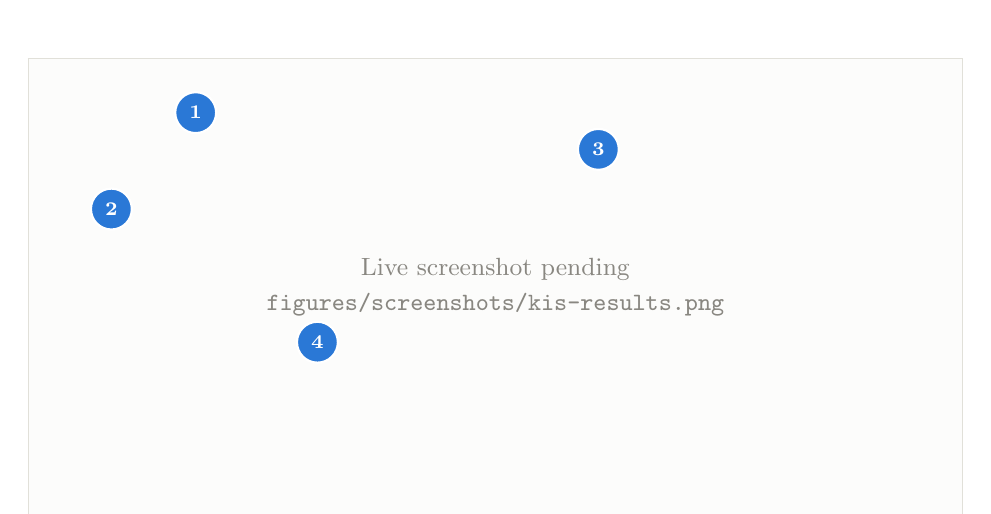
\begin{tikzpicture}
  \node[anchor=south west,inner sep=0] (image) at (0,0)
    {\screenshotplaceholder{figures/screenshots/kis-results.png}{0.96\textwidth}};
  \begin{scope}[x={(image.south east)},y={(image.north west)}]
    \node[callout] at (0.18,0.88) {1};
    \node[callout] at (0.09,0.67) {2};
    \node[callout] at (0.61,0.80) {3};
    \node[callout] at (0.31,0.38) {4};
  \end{scope}
\end{tikzpicture}
\caption{KIS retrieval workspace. \calloutlabel{1} Natural-language query and mode-sensitive input; \calloutlabel{2} Top-$K$, dense/BM25 controls, and shared answer files; \calloutlabel{3} latency and result summary; \calloutlabel{4} canonical result cards with an expanded event alignment and submission action.}
\label{fig:ui-kis}
\end{figure}

\begin{figure}[htbp]
\centering
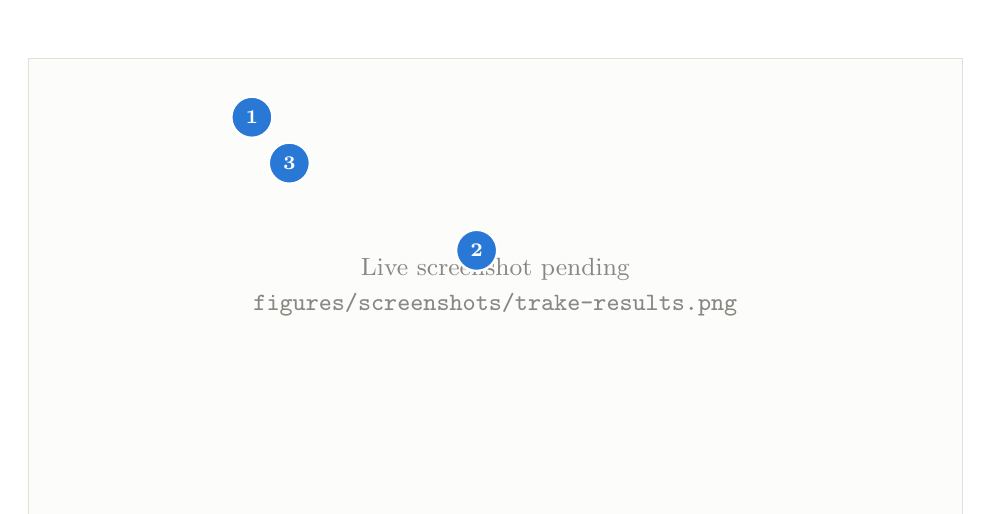
\begin{tikzpicture}
  \node[anchor=south west,inner sep=0] (image) at (0,0)
    {\screenshotplaceholder{figures/screenshots/trake-results.png}{0.96\textwidth}};
  \begin{scope}[x={(image.south east)},y={(image.north west)}]
    \node[callout] at (0.24,0.87) {1};
    \node[callout] at (0.48,0.58) {2};
    \node[callout] at (0.28,0.77) {3};
  \end{scope}
\end{tikzpicture}
\caption{TRAKE ordered-event retrieval. \calloutlabel{1} Sequential \code{E1..En} specification; \calloutlabel{2} one same-video path displayed in event order; \calloutlabel{3} path-level submission action, which emits one ordered multi-frame CSV row rather than independent frame submissions.}
\label{fig:ui-trake}
\end{figure}

\begin{figure}[htbp]
\centering
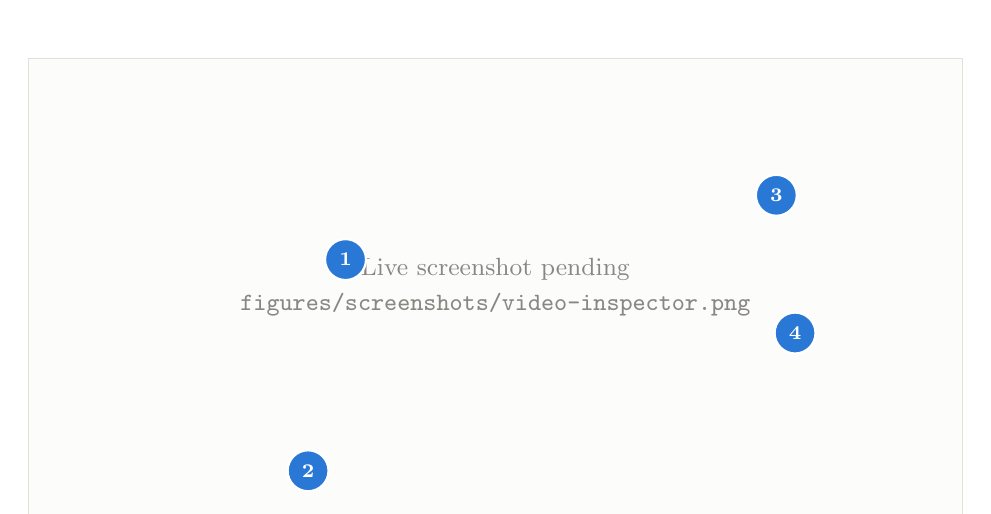
\begin{tikzpicture}
  \node[anchor=south west,inner sep=0] (image) at (0,0)
    {\screenshotplaceholder{figures/screenshots/video-inspector.png}{0.96\textwidth}};
  \begin{scope}[x={(image.south east)},y={(image.north west)}]
    \node[callout] at (0.34,0.56) {1};
    \node[callout] at (0.30,0.10) {2};
    \node[callout] at (0.80,0.70) {3};
    \node[callout] at (0.82,0.40) {4};
  \end{scope}
\end{tikzpicture}
\caption{Video evidence inspector. \calloutlabel{1} media preview positioned at the retrieved moment; \calloutlabel{2} custom timeline and precise seek controls; \calloutlabel{3} live canonical/submission coordinates; \calloutlabel{4} available caption, OCR, object, and other inspectable evidence used for human verification.}
\label{fig:ui-player}
\end{figure}

\begin{figure}[htbp]
\centering
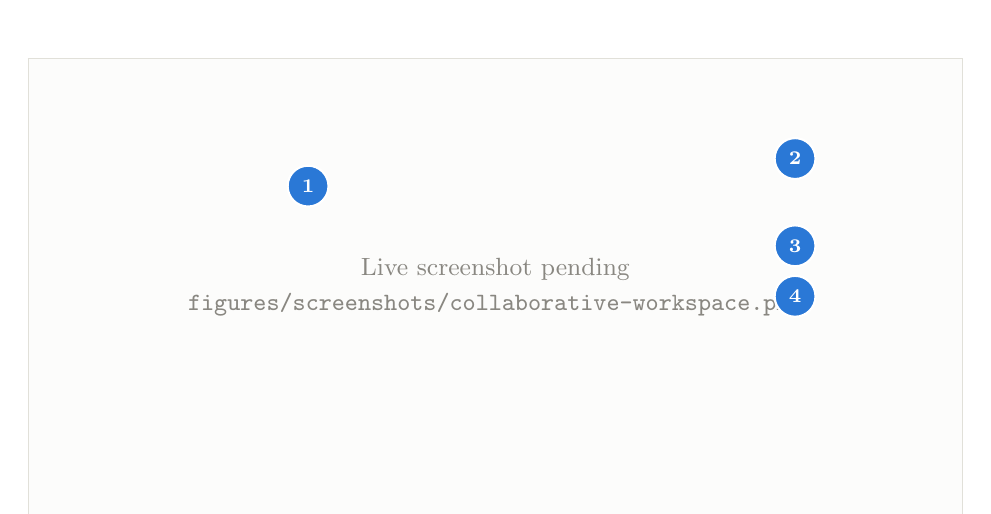
\begin{tikzpicture}
  \node[anchor=south west,inner sep=0] (image) at (0,0)
    {\screenshotplaceholder{figures/screenshots/collaborative-workspace.png}{0.96\textwidth}};
  \begin{scope}[x={(image.south east)},y={(image.north west)}]
    \node[callout] at (0.30,0.72) {1};
    \node[callout] at (0.82,0.78) {2};
    \node[callout] at (0.82,0.59) {3};
    \node[callout] at (0.82,0.48) {4};
  \end{scope}
\end{tikzpicture}
\caption{Collaborative Workspace. \calloutlabel{1} user-scoped query history and replay; \calloutlabel{2} manual video/timestamp opening; \calloutlabel{3} shared SQLite-backed submission files with distinct validated and filled states; \calloutlabel{4} multi-file CSV ZIP export.}
\label{fig:ui-workspace}
\end{figure}

\clearpage
\section{Traceability and Deployment Evidence}

\begin{table}[htbp]
\centering
\caption{Coverage matrix for every subsystem presented in the four-page body. UI behavior is evidenced by a live capture; nonvisual computation is evidenced by a diagram and/or manifest table.}
\label{tab:coverage}
\small
\begin{tabularx}{\textwidth}{@{}>{\bfseries}p{0.22\textwidth}Xp{0.30\textwidth}@{}}
\toprule
Presented subsystem & Appendix evidence & Primary implementation boundary \\
\midrule
End-to-end architecture / services & Fig.~\ref{fig:architecture}; Table~\ref{tab:models} & \pathcode{src/hcmai/orchestration}, \pathcode{src/hcmai/app.py}, \pathcode{llm/} \\
Keyframe ingestion / identity & Fig.~\ref{fig:preparation}; Table~\ref{tab:parameters} & \pathcode{offline/keyframes}, \pathcode{offline/ingestion} \\
Caption, OCR, objects, ASR, FrameContext & Fig.~\ref{fig:preparation}; Tables~\ref{tab:models}--\ref{tab:artifacts} & \pathcode{offline/enrichment/context} \\
FAISS / BM25 / fusion & Figs.~\ref{fig:preparation} and~\ref{fig:temporal}; Tables~\ref{tab:artifacts}--\ref{tab:parameters} & \pathcode{src/hcmai/retrieval} \\
Temporal DP / KIS / TRAKE & Figs.~\ref{fig:temporal} and~\ref{fig:dp-explainer} & \pathcode{src/hcmai/temporal}, \pathcode{orchestration/workflows} \\
KIS operator flow & Fig.~\ref{fig:ui-kis} & \pathcode{frontend/src/features/search} \\
TRAKE operator flow & Fig.~\ref{fig:ui-trake} & \pathcode{frontend/src/features/search/Trake*} \\
Video preview / evidence inspection & Fig.~\ref{fig:ui-player} & \pathcode{frontend/src/features/frames} \\
Collaborative workspace / submissions & Fig.~\ref{fig:ui-workspace} & \pathcode{frontend/src/features/workspace}, \pathcode{features/submission} \\
Thunder Compute / S3 execution & Fig.~\ref{fig:architecture}; text below & \pathcode{scripts/build_retrieval_indexes.py}, \pathcode{llm/server} \\
\bottomrule
\end{tabularx}
\end{table}

\begin{figure}[htbp]
\centering
\resizebox{0.98\textwidth}{!}{%
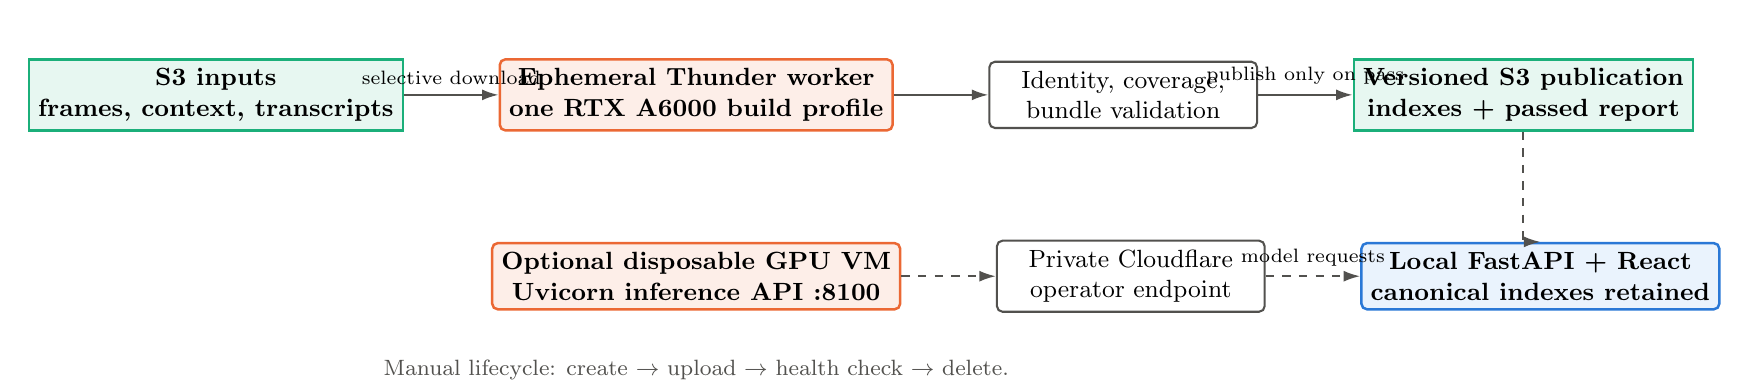
\begin{tikzpicture}[node distance=8mm and 10mm]
  \node[artifact,minimum width=35mm] (s3in) {S3 inputs\\frames, context, transcripts};
  \node[service,minimum width=41mm,right=12mm of s3in] (a6000) {Ephemeral Thunder worker\\one RTX A6000 build profile};
  \node[process,minimum width=34mm,right=12mm of a6000] (validate) {Identity, coverage,\\bundle validation};
  \node[artifact,minimum width=40mm,right=12mm of validate] (s3out) {Versioned S3 publication\\indexes + passed report};
  \draw[flowarrow] (s3in) -- node[above,font=\scriptsize]{selective download} (a6000);
  \draw[flowarrow] (a6000) -- (validate);
  \draw[flowarrow] (validate) -- node[above,font=\scriptsize]{publish only on pass} (s3out);

  \node[service,minimum width=41mm,below=14mm of a6000] (vm) {Optional disposable GPU VM\\Uvicorn inference API :8100};
  \node[process,minimum width=34mm,right=12mm of vm] (edge) {Private Cloudflare\\operator endpoint};
  \node[client,minimum width=40mm,right=12mm of edge] (local) {Local FastAPI + React\\canonical indexes retained};
  \draw[dataarrow] (vm) -- (edge);
  \draw[dataarrow] (edge) -- node[above,font=\scriptsize]{model requests} (local);
  \draw[dataarrow] (s3out.south) |- (local.north);
  \node[note,below=5mm of vm,anchor=north] {Manual lifecycle: create $\rightarrow$ upload $\rightarrow$ health check $\rightarrow$ delete.};
\end{tikzpicture}%
}
\caption{Thunder Compute execution modes. Index construction and optional online inference are separate lifecycles. Canonical serving artifacts are versioned outside the VM, so deleting a GPU instance does not delete retrieval state.}
\label{fig:thunder}
\end{figure}

\paragraph{Release note.}
The runbook's pass-gated publication contract is the intended deployment policy.
The local snapshot documented in Table~\ref{tab:artifacts} does not contain the
promoted build report and has incomplete visual/context provenance fields; those
must be reconciled before an official immutable-bundle claim. The inference
example also demonstrates an L40 while the index-build profile specifies an
A6000. Figure~\ref{fig:thunder} therefore labels GPU choice by workflow rather
than conflating the examples.


\end{document}
